\documentclass[tikz,border=10pt]{standalone}
\usepackage{amsmath}
\definecolor{bg}{HTML}{171D2B}
\definecolor{aksen}{HTML}{F7B538}
\definecolor{isibg}{HTML}{2A3550}
\begin{document}
\pagecolor{bg}
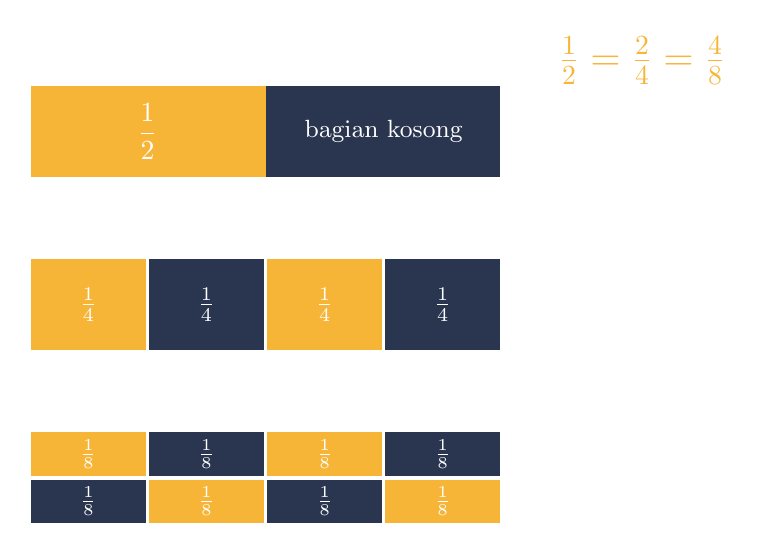
\begin{tikzpicture}[scale=1.0]
\begin{scope}
\fill[isibg] (0,0) rectangle (6,1.2);
\fill[aksen] (0,0) rectangle (3,1.2);
\draw[white,line width=1.2pt] (0,0) rectangle (6,1.2);
\node[white] at (1.5,0.6) {$\dfrac{1}{2}$};
\node[white] at (4.5,0.6) {\small bagian kosong};
\end{scope}
\begin{scope}[yshift=-2.2cm]
\fill[isibg] (0,0) rectangle (6,1.2);
\fill[aksen] (0,0) rectangle (1.5,1.2);
\fill[aksen] (3,0) rectangle (4.5,1.2);
\draw[white,line width=1.2pt] (0,0) rectangle (6,1.2);
\foreach \x in {1.5,3,4.5} \draw[white,line width=1.2pt] (\x,0) -- (\x,1.2);
\node[white] at (0.75,0.6) {$\frac{1}{4}$};
\node[white] at (2.25,0.6) {$\frac{1}{4}$};
\node[white] at (3.75,0.6) {$\frac{1}{4}$};
\node[white] at (5.25,0.6) {$\frac{1}{4}$};
\end{scope}
\begin{scope}[yshift=-4.4cm]
\fill[isibg] (0,0) rectangle (6,1.2);
\foreach \i/\j in {0/0,1/0,2/0,3/0,0/1,1/1,2/1,3/1} {
  \pgfmathsetmacro{\x}{\i*1.5}
  \pgfmathsetmacro{\y}{\j*0.6}
  \ifodd\numexpr\i+\j\relax
    \fill[aksen] (\x,\y) rectangle (\x+1.5,\y+0.6);
  \fi
}
\draw[white,line width=1.2pt] (0,0) rectangle (6,1.2);
\foreach \x in {1.5,3,4.5} \draw[white,line width=1.2pt] (\x,0) -- (\x,1.2);
\draw[white,line width=1.2pt] (0,0.6) -- (6,0.6);
\foreach \x/\lab in {0.75/1,2.25/2,3.75/3,5.25/4} {
  \node[white] at (\x,0.3) {\footnotesize $\frac{1}{8}$};
  \node[white] at (\x,0.9) {\footnotesize $\frac{1}{8}$};
}
\end{scope}
\node[aksen,right] at (6.6,1.5) {\Large $\frac{1}{2}=\frac{2}{4}=\frac{4}{8}$};
\end{tikzpicture}
\end{document}
